\chapter{Related Work}
\label{chap:lit}

This dissertation lies at the intersection of language testing, second language acquisition (SLA), intelligent computer-assisted language learning (ICALL), corpus linguistics and natural language processing (NLP). My work here is much indebted to related research in these areas, and this chapter will summarize some of the most relevant studies.

\lk{Maybe it's better to have a P here summarizing my ``ethos'' (low resource, content focused, interpretable) instead of spreading that out below.}

I begin in Section~\ref{section:ICALLinterp} with a discussion of the importance of transparency and interpretability in ICALL and language testing. In  Section~\ref{section:ICALLoverview}, I examine approaches to ICALL that relate to and inform this dissertation. In Section~\ref{section:learnerCorpora}, I summarize research involving the collection, annotation or content analysis of task-based learner corpora. A brief overview of the NLP tools and methods used in my work is given in Section~\ref{section:NLP}. Finally, in Section~\ref{section:myPreviousWork}, I present a summary of my own previous work related to this dissertation. 

\section{On interpretability for learner applications}
\label{section:ICALLinterp}
This work would be remiss without discussing the role of machine learning (ML) in current NLP, given that such technologies are largely absent from this dissertation. Recent years have seen the rapid development of ML technologies like neural networks and deep learning. \lk{What is ML good at? citations!} These technologies have been widely implemented in areas like NLP and computer vision, often with impressive gains in performance. They can also lead to reductions in the amount of human expertise needed to automate tasks like syntactic labeling, voice recognition and synthesis, and object and facial recognition. \lk{cite stuff} Naturally, this also means significant reductions in the cost of such systems. A major drawback with many such ML technologies, however is the loss of interpretability. For example, \textit{word embeddings} (such as Word2Vec) \lk{cite} are ML based NLP tools suitable for many tasks involving the processing of linguistic meaning or structures. Word2Vec essentially ``learns'' an approximation of the meanings and grammatical usage of words by observing them in context. Instead of relying on expert annotation of features like part-of-speech, sentence structure and morphology to train a model, the system needs only large amounts of raw text. From this text, it observes large numbers of features, such as the average distance between instances of \textit{Word A} and \textit{Word B}. It reduces these raw features to a (still quite large) number of abstract features, or ``latent variables'', which form a vector of numeric values; this vector then serves as a representation of a word's ``meaning''. In a classic example, if one takes the vector for ``queen'', subtracts the vector for ``female'' and adds the vector for ``male'', the resulting vector is roughly equivalent to that of ``king''.

\lk{this is all very cf Brian Riordan's alumni talk... similar sources would be ideal}
For many applications, the capabilities and cost reduction of ML make it an attractive and suitable choice; this is certainly the case with many NLP tasks. The use of ML tools with learner language is problematic on at least two fronts, however. First, such tools are typically designed for and trained on well-formed, native-like text (or speech). As mentioned, these tools generally do not rely on annotation in their training data; instead, they make up for this lack of expertise by the sheer volume of training data they consume. Including real learner data on the scale required by ML tools would be impractical if not impossible for most researchers. As a result of ML tools' training on mostly native-like data, they are ill-equipped for processing the variability and ambiguity of learner language. For example, native English trained NLP tools expect regular sentence punctuation; text from a beginning English learner lacking in punctuation could therefore be misconstrued as having longer sentences and thus higher proficiency \cite{MeurersDickinson2017}. Second, and perhaps more importantly, tools that rely heavily on ML are inherently less interpretable than ``classical'' NLP tools. Because classical NLP tools are trained on expert annotation, their output is generally determined by the kinds of features that are annotated in the training corpus. This means linguistic researchers can design NLP tools and pipelines that produce output precisely suited for their research questions, so long as they have the resources to produce adequate training corpora. This is not the case with ML based tools, however. Due to their reliance on abstract features and latent variables, these newer tools are largely ``black box'' technologies; raw data goes in and processed data comes out, but even the architect of such a system cannot explain exactly how or why the analysis was produced. In a language learning application, this is problematic because it means the development of a pedagogically sound feedback system for the learner is not possible; the features underlying the analysis are not accessible or interpretable. The outcomes of language testing can have a tremendous impact on a test taker's future, and in such a high stakes application, the lack of interpretability can be even more problematic. Arguably, it is far better for all stakeholders if a language test can deliver not only a score, but also a rationale for that score, such as which kinds of errors a test taker makes and in what contexts. This need for interpretable features was one of a few major factors in the decision to choose classical NLP over newer ML tools in this dissertation, and most of the related studies discussed here take similar approaches.

\section{An overview of ICALL and content analysis}
\label{section:ICALLoverview}
This dissertation began as an experiment in bootstrapping NLP tools and learner data to achieve more meaning-based (and meaningful) ICALL. I do not attempt a full-fledged ICALL system, but I explore mechanisms for performing the core content analysis that could be implemented in a setting like a game, an interactive language tutor (ILT) or a language test. I see this work as a push toward relatively low-cost, extendable ICALL with an emphasis on content over form. Each of these points is an attempt at a more interdisciplinary and pedagogically sound approach to ICALL. In keeping with this ethos, this section focuses on ICALL research that primarily uses existing NLP tools and allows for free user input (as opposed to menu-based input).

One relatively well-documented ICALL system is TAGARELA, an application for adult learners of Portuguese \cite{amaral2007designing,amaral:meurers:user:07}. In more recent updates to the system, the authors describe TAGARELA's ``Unstructured Information Management Architecture (UIMA),'' which is effectively a collection of text relevant to the tasks that are enriched with multiple annotations relating to both form and meaning. TAGARELA relies on a set of NLP modules implemented in a flexible, task-based, free input ICALL system \cite{Amaral.Meurers.Ziai-11}. The system includes six different activity types: reading, listening, description, rephrasing, vocabulary and fill-in-the-blank. These different tasks require different types of (textual) learner input as well as different subsets of the NLP modules for input processing and the generation of feedback.

Before developing anything, the TAGARELA team began their work with the creation of a ``taxonomy of expected errors,'' gleaned from their analysis of a corpus of written assignments from learners of Portuguese. The authors describe their approach as ``data-driven rather than process-driven''. In many ways, this bucks a tendency among many ICALL developers to simply address the kinds of errors NLP tools can readily identify. \lk{cite DuoLingo? etc.}What is needed instead is ICALL development informed by second language acquisition research and by the kinds of challenges learners face, as borne out by real data. \lk{cite Ellis, Meurers}These errors annotated in the learner data and handled by TAGARELA cover both form and meaning, with error types consisting of, for example, \textit{spelling}, \textit{agreement} and \textit{word choice}.

One major advantage of TAGARELA's approach to ICALL is its ability to accommodate multiple activities with only a handful of existing and custom NLP modules along with a small number of carefully chosen and annotated model responses. The current dissertation found inspiration in TAGARELA's prioritization of the handling of errors related to meaning and its reliance on ordinary and interpretable NLP tools -- primarily a tokenizer, part of speech tagger and syntactic parser. 

\section{Learner corpora}
\label{section:learnerCorpora}
Here I will discuss task-based learner corpora research that relates to my work. This includes discussions of task design, data collection, annotation schemes, and automatic processing. I focus in particular on the learner content analysis research conducted by two clusters of researchers: one primarily associated with The Ohio State University and consisting of Detmar Meurers and colleagues, and the other primarily associated with Educational Testing Services (ETS) and consisting of Martin Chodorow, Swapna Somasundaran and Joel Tetrault and colleagues. 

Here are some papers I discussed briefly in my BEA 2018 paper:

\cite{leacock:ea:14}

\cite{kyle2015automatically}

\cite{weigle2013english}

\cite{amaral:meurers:user:07}

\cite{Meurers.Dickinson-17}

\cite{heift:schulze:07}

\cite{somasundaran:ea:15}

\cite{bailey:meurers:08}

\cite{meurers2011evaluating}

\cite{somasundaran:chodorow:14}

\cite{cahill-et-al:14}

\cite{ragheb:dickinson:14a}

\cite{foster2009native}

\cite{cho2013investigating}

\cite{landis1977measurement}

\cite{artstein:massimo:2008}

\cite{tetreault-chodorow:2008:HJCL}

\cite{tetreault:chodorow:08}

\section{Language assessment}
\label{section:languageAssessment}

\section{NLP tools and methods}
\label{section:NLP}

\section{My previous work}
\label{section:myPreviousWork}
Here I will discuss the work I have previously done in this area, including the papers given in the subsections below.

\subsection{2013}
\cite{king:dickinson:13}

\begin{figure}
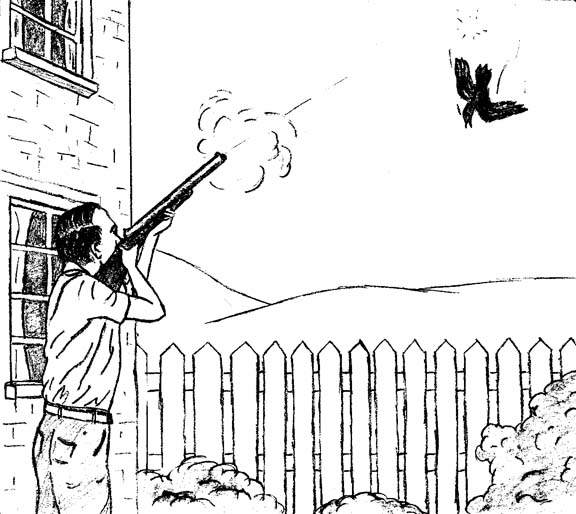
\includegraphics[width=.7\textwidth]{figures/exampleprompt2.jpg}
\caption{This is an example figure from \citet{king:dickinson:13}.}
\label{figure:KandD2013}
\end{figure}

\subsection{2014}
\citet{king:dickinson:14}

\subsection{2016}
\citep{king:dickinson:16}

\subsubsection{Bag-of-dependencies}
Here we could discuss the switch to a bag-of-dependencies approach, the use of tf-idf and the use of vector cosine distance for ranking responses.

\subsubsection{Clustering}
Here we could briefly mention the clustering experiments we did in the 2016 paper. But really, I'd rather not, because I don't intend to repeat them in the dissertation.

\subsection{2018}
\cite{king:dickinson:18}

\begin{figure}

\includegraphics[width=.7\textwidth]{figures/I29.jpg}
\caption{This is an example figure from \citet{king:dickinson:18}.}
\label{figure:KandD2018}
\end{figure}

\section{Image processing}
\label{figure:imageProcessing}
We want to touch on image processing / automatic captioning / use of semantic primatives, etc. -- linguistic annotation of images. NOT a deep discussion, but we need to acknowledge that there are other fields working on the relations between images and text, and give an idea of what some approaches are and how they work, and how they might relate to my work and the work discussed in my lit review.


% This is a figure in landscape orientation
%\begin{sidewaysfigure}
%
\includegraphics[width=\textwidth]{figures/exampleFigure.png}
%\caption{This is another example Figure, rotated to landscape orientation.}
%\label{LandscapeFigure}
%\end{sidewaysfigure}
